\documentclass[border=10pt]{standalone}

\usepackage{tikz}
\usepackage{tikzsymbols}
\usetikzlibrary{calc,patterns,shapes.geometric}

\def\centerarc[#1](#2)(#3:#4:#5){\draw[#1] ($(#2)+({#5*cos(#3)},{#5*sin(#3)})$) arc (#3:#4:#5);}

\begin{document}
	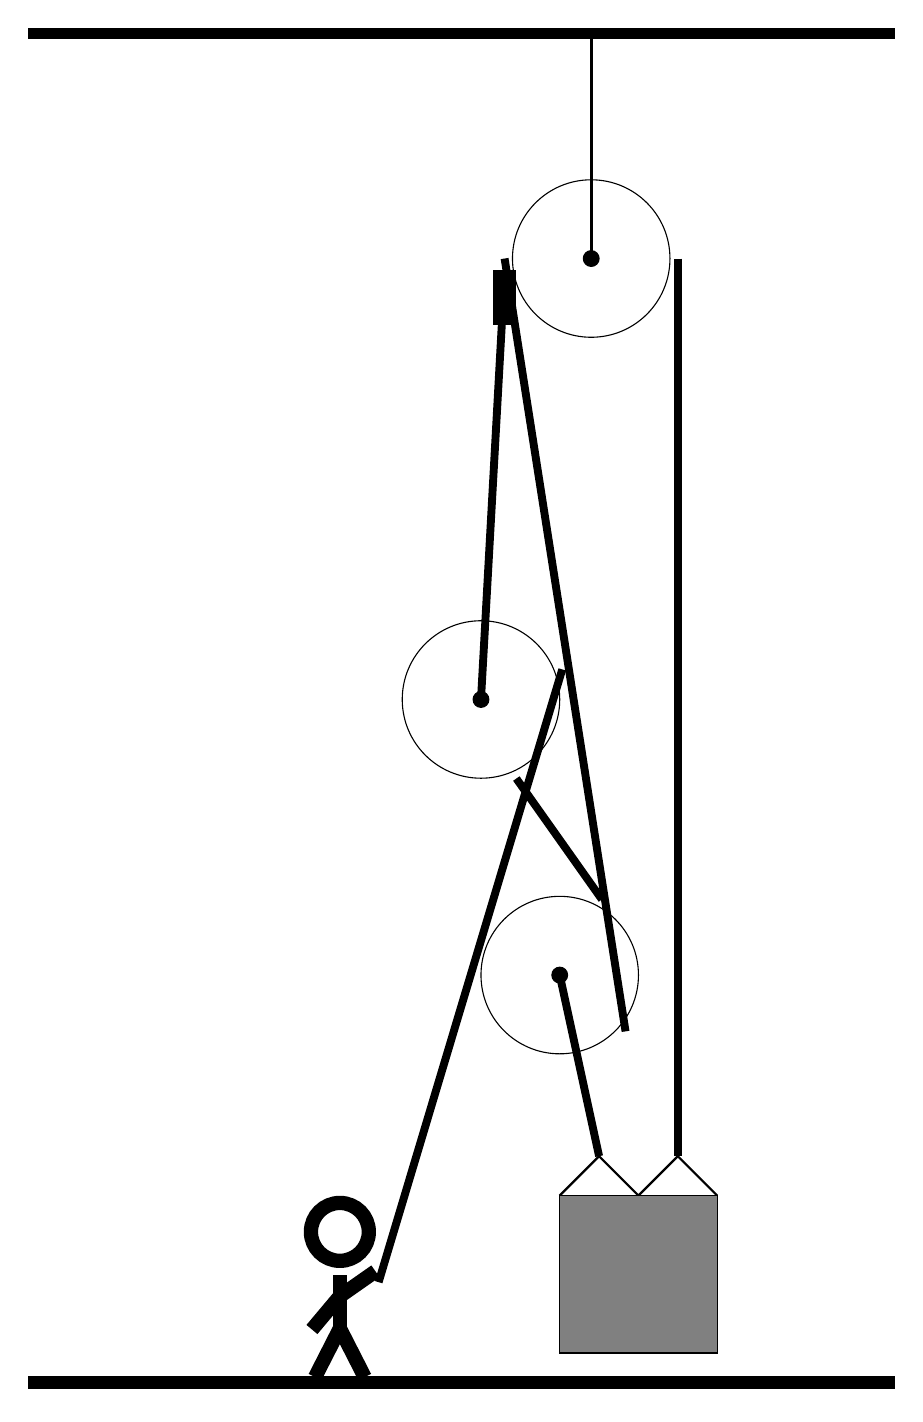
\begin{tikzpicture}
		%%%%% START %%%%%
		\draw[fill=black] (-6, 14) rectangle (5, 14.125);
		
		\draw (-0.25, 5.6) circle (1);
		\draw[fill=black] (-0.25, 5.6) circle (0.1);
		
		\draw (0.75, 2.1) circle (1);
		\draw[fill=black] (0.75, 2.1) circle (0.1);
		
		\draw (1.15, 11.2) circle (1);
		\draw[fill=black] (1.15, 11.2) circle (0.1);
		\draw[very thick] (1.15, 11.2) -- (1.15, 14);
		
		\draw[thick]  (0.75, -0.7) -- (1.25, -0.2) -- (1.75, -0.7) -- (2.25, -0.2) -- (2.75, -0.7);
		\draw[fill=black!50] (0.75, -0.7) rectangle (2.75, -2.7);
		
		\draw[line width=1mm] (-0.25, 5.6) -- (0.05, 11.0);
		\draw[line width=1mm, fill=black](-0.05, 10.4) rectangle (0.15, 11.0);
		\draw[line width=1mm] (-1.55, -1.8) -- (0.782, 5.982);
		\centerarc[line width=1mm](-0.25, 5.6)(-20:170:1.1);
		\draw[line width=1mm] (0.199, 4.596) -- (1.286, 3.06);
		\centerarc[line width=1mm](0.75, 2.1)(160:380:1.1);
		\draw[line width=1mm] (1.586, 1.385) -- (0.05, 11.2);
		\draw[line width=1mm](0.75, 2.1) -- (1.25, -0.2);
		\centerarc[line width=1mm](1.15, 11.2)(0:180:1.1);
		\draw[line width=1mm] (2.25, 11.2) -- (2.25, -0.2);
		
		\node at (-2, -1.9) {\Strichmaxerl[10][50][35]};
		
		\draw[fill=black] (-6, -3) rectangle (5, -3.15);
		%%%%% END %%%%%
	\end{tikzpicture}
\end{document}